\documentclass{beamer}

\usepackage{graphicx}
\usepackage{graphicx}
\usepackage{pgffor}
\usepackage{hyperref}



\setbeamertemplate{navigation symbols}{}
\usetheme{Montpellier}


\begin{document}

\author{by Eszter Domokos-Kővári  \\  \tiny }
	
\title{Karinthy} 

\setlength{\parindent}{1em}



    \begin{frame}
    \maketitle
    \end{frame}




\section{Citations}


\begin{frame}

\frametitle {Citations}

   \begin{itemize}
\item   ``Humorban nem ismerek tréfát. `` \par 

\item   ``Lehet-e őszinte barátság férfi és nő között, igen vagy nem, és ha igen, miért nem?`` \par 

\item   ``A kormány az a testület, ami mindig megtartja, amit ígér. Ha pénzt ígér, azt is megtartja. `` \par 

\item   ``Férfi és nő. Hogy érthetnék meg egymást? Hisz mind a kettő mást akar - a férfi nőt - a nő férfit. `` \par 

\item   ``A lelki sérülés nem múlik el soha. De hozzáedződik a lélek. `` \par 
    \end{itemize}

    \end{frame}

\begin{frame} 
 
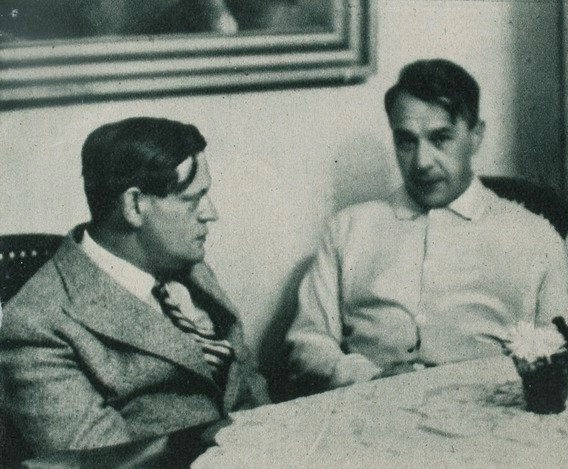
\includegraphics[ width=3cm]{KUndK.jpg}

   \begin{itemize}
\item   ``Hisztéria. Veszedelmes betegség, kötelezően kellene gyógyítani. Csak nők kaphatják meg, és csak férfiak halnak bele. `` \par 

\item   ``Ha egyedül vagyok egy szobában, akkor ember vagyok. Ha bejön egy nő, akkor férfi lettem. És annyira vagyok férfi, amennyire nő az, aki bejött a szobába. `` \par 

\item   ``Az emberekben nem lehet megbízni... a legjobbakban is csalódunk, akikről semmi okunk nem volt hinni, hogy keserűséget, bánatot és csalódást okoznak nekünk... talán jóhiszeműen vagy tudaton kívül? Meglehet, de ez nem változtat semmit a kínos megdöbbenésen. `` \par 



    \end{itemize}
    \end{frame}

\begin{frame} 
 
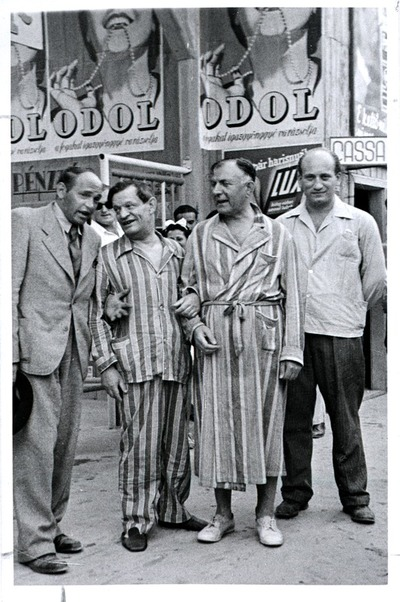
\includegraphics[ width=2.5cm]{Team.jpg};
   \begin{itemize}
\item   ``Születni és meghalni lehet egy nap alatt - de élni nem. `` \par 

\item   ``A szerelem egyenlet két ismeretlennel. `` \par 

\item   ``Jobb lett volna meg sem születni
Nékünk, mint egymást nem szeretni. `` \par 

    \end{itemize}
    \end{frame}

\begin{frame} 

   \begin{itemize}

\item   ``Házasság. Megállapodás férfi és nő közt, melyben kölcsönösen szerződnek, hogy nem mondják el egymásnak, hogy ki tetszik nekik.`` \par 

\item   ``Emlékezz rá, hogy egyszer még, utoljára, találkoztál velem... És ha van még benned valami belőlem, mártsd be tolladat a lenyugvó nap tüzébe, s írd meg nekik... írd meg ezt a találkozást... és írd meg nekik, hogy hagytalak el, és hogy tűntem el, beleolvadva az alkonyodó égbe, ifjan, szépen és végtelenül szabadon, hogy ne lássalak többé.  `` \par 

\item   ``Nem értünk rá tanulni, mert folyton tanítottak.``
    \end{itemize}

\medskip 
  ``Az álmodó, aki tudja, hogy csak álmodik, félig ébren van már.`` \par  

\end{frame}

\section{Animation}


\foreach \index in {1, ..., 5} 
	{
	\begin{frame}
    	\begin{center}
  	\includegraphics[width=\textwidth]{Frici\index.png}\par%
	\end{center}
	\end{frame}
  	}



\end{document}